\documentclass[a4paper,14pt]{extarticle} %,twoside

%%%%%%%%%%%%%%%%%%%%%%%%%%%%%%%%%%%%%%%%%%%%%%%%%%%%%%
%%%% Файл упрощённых настроек шаблона диссертации %%%%
%%%%%%%%%%%%%%%%%%%%%%%%%%%%%%%%%%%%%%%%%%%%%%%%%%%%%%

%%%        Подключение пакетов                 %%%
\usepackage{ifthen}                 % добавляет ifthenelse
%%% Инициализирование переменных, не трогать!  %%%
\newcounter{intvl}
\newcounter{otstup}
\newcounter{contnumeq}
\newcounter{contnumfig}
\newcounter{contnumtab}
\newcounter{pgnum}
\newcounter{bibliosel}
\newcounter{chapstyle}
\newcounter{headingdelim}
\newcounter{headingalign}
\newcounter{headingsize}
\newcounter{tabcap}
\newcounter{tablaba}
\newcounter{tabtita}
%%%%%%%%%%%%%%%%%%%%%%%%%%%%%%%%%%%%%%%%%%%%%%%%%%

%%% Область упрощённого управления оформлением %%%

%% Интервал между заголовками и между заголовком и текстом
% Заголовки отделяют от текста сверху и снизу тремя интервалами (ГОСТ Р 7.0.11-2011, 5.3.5)
\setcounter{intvl}{3}               % Коэффициент кратности к размеру шрифта

%% Отступы у заголовков в тексте
\setcounter{otstup}{0}              % 0 --- без отступа; 1 --- абзацный отступ

%% Нумерация формул, таблиц и рисунков
\setcounter{contnumeq}{0}           % Нумерация формул: 0 --- пораздельно (во введении подряд, без номера раздела); 1 --- сквозная нумерация по всей диссертации
\setcounter{contnumfig}{0}          % Нумерация рисунков: 0 --- пораздельно (во введении подряд, без номера раздела); 1 --- сквозная нумерация по всей диссертации
\setcounter{contnumtab}{1}          % Нумерация таблиц: 0 --- пораздельно (во введении подряд, без номера раздела); 1 --- сквозная нумерация по всей диссертации

%% Оглавление
\setcounter{pgnum}{1}               % 0 --- номера страниц никак не обозначены; 1 --- Стр. над номерами страниц (дважды компилировать после изменения)

%% Библиография
\setcounter{bibliosel}{0}           % 0 --- встроенная реализация с загрузкой файла через движок bibtex8; 1 --- реализация пакетом biblatex через движок biber

%% Текст и форматирование заголовков
\setcounter{chapstyle}{1}           % 0 --- разделы только под номером; 1 --- разделы с названием "Глава" перед номером
\setcounter{headingdelim}{1}        % 0 --- номер отделен пропуском в 1em или \quad; 1 --- номера разделов и приложений отделены точкой с пробелом, подразделы пропуском без точки; 2 --- номера разделов, подразделов и приложений отделены точкой с пробелом.

%% Выравнивание заголовков в тексте
\setcounter{headingalign}{0}        % 0 --- по центру; 1 --- по левому краю

%% Размеры заголовков в тексте
\setcounter{headingsize}{0}         % 0 --- по ГОСТ, все всегда 14 пт; 1 --- пропорционально изменяющийся размер в зависимости от базового шрифта

%% Подпись таблиц
\setcounter{tabcap}{0}              % 0 --- по ГОСТ, номер таблицы и название разделены тире, выровнены по левому краю, при необходимости на нескольких строках; 1 --- подпись таблицы не по ГОСТ, на двух и более строках, дальнейшие настройки: 
%Выравнивание первой строки, с подписью и номером
\setcounter{tablaba}{2}             % 0 --- по левому краю; 1 --- по центру; 2 --- по правому краю
%Выравнивание строк с самим названием таблицы
\setcounter{tabtita}{1}             % 0 --- по левому краю; 1 --- по центру; 2 --- по правому краю

%%% Цвета гиперссылок %%%
% Latex color definitions: http://latexcolor.com/
\definecolor{linkcolor}{rgb}{0.9,0,0}
\definecolor{citecolor}{rgb}{0,0.6,0}
\definecolor{urlcolor}{rgb}{0,0,1}
\definecolor{linkcolor}{rgb}{0,0,0} %black
\definecolor{citecolor}{rgb}{0,0,0} %black
%\definecolor{urlcolor}{rgb}{0,0,0} %black               % Упрощённые настройки шаблона 

%%% �������� �������� %%%
\newcommand{\thesisAuthor}             % �����������, ��� ������
{\texorpdfstring{\todo{����� ��� ����}}{������� ��� �������� ������}}  % \texorpdfstring takes two arguments and uses the first for (La)TeX and the second for pdf
\newcommand{\thesisUdk}                % �����������, ���
{\todo{xxx.xxx}}
\newcommand{\thesisTitle}              % �����������, ��������
{\texorpdfstring{\todo{\MakeUppercase{%���������� ������������ ������� � ������� ������������� �������� � �������� ��������� ������
%���������� ������������ ������� ��������� � ���������� ������� ������������� �������� ������������ ������}}}{�������� ��������������� ������}}
%������������ ������ ���������: \newline ������ � ���������� � ������������� �������� ������������ ������}}}{�������� ��������������� ������}}
%������������ ��������� ���������: ������ � ���������� � ������������� �������� ������������ ������}}}{�������� ��������������� ������}}
%������������ ��������� ���������: ��������� ������ � ���������� � ������������� �������� ������������ ������}}}{�������� ��������������� ������}}
%����������� ��������� ���������� � ��������� �������������� �� ����� ������� �������� � ������ �� ������ ������������ ������� ���������}}}{�������� ��������������� ������}}
%����������� ��������� ���������� � ��������� �������������� �� ������ ������������ ������� ���������}}}{�������� ��������������� ������}}
%����������� ��������� ��������������� �������������� �� ������ ������������ ������� ���������}}}{�������� ��������������� ������}}
���������� � ���������� ���������� ������������� ������ � ������ �������������}}}{�������� ��������������� ������}}
%���������� ������������ ������� ��������� � ����������� ��������� ���������� � ��������� �������������� �� ����� ������� ��������}}}{�������� ��������������� ������}}
\newcommand{\thesisSpecialtyNumber}    % �����������, �������������, �����
{\texorpdfstring{\todo{05.13.18}}{XX.XX.XX}}
\newcommand{\thesisSpecialtyTitle}     % �����������, �������������, ��������
{\texorpdfstring{\todo{�������������� �������������, ��������� ������ � ��������� ��������}}{�������� �������������}}
\newcommand{\thesisDegree}             % �����������, ������� �������
{\todo{
%��������� ������-�������������� ����
��������� ����������� ����
}}
\newcommand{\thesisCity}               % �����������, ����� ������
{\todo{�������}}
\newcommand{\thesisYear}               % �����������, ��� ������
{\todo{2017}}
\newcommand{\thesisOrganization}       % �����������, �����������
{\todo{��������� ������������ ����������������� ����������� �����������}}

\newcommand{\thesisInOrganization}       % �����������, ����������� � ���������� ������: ������ ��������� � ...
{\todo{��������� ������������ ����������������� ����������� ������������}}

\newcommand{\supervisorFio}            % ������� ������������, ���
{\todo{������� ����� ����������}}
\newcommand{\supervisorRegalia}        % ������� ������������, �������
{\todo{������ ������-�������������� ����, ������}}

\newcommand{\opponentOneFio}           % �������� 1, ���
{\todo{������� ��� ��������}}
%{\todo{������������� ���� ����������}}
\newcommand{\opponentOneRegalia}       % �������� 1, �������
{\todo{������ ������-�������������� ����, ���������}}
\newcommand{\opponentOneJobPlace}      % �������� 1, ����� ������
%{\todo{��������� ��������������� ������������-������������ �����������}}
{\todo{�� ����� ������� �������� ��� ����� ������}}
\newcommand{\opponentOneJobPost}       % �������� 1, ���������
%{\todo{���. ���. ���������� ����������}}
{\todo{������� ������� ���������}}

\newcommand{\opponentTwoFio}           % �������� 2, ���
{\todo{������� ��� ��������}}
%{\todo{��������� ����� ����������}}
\newcommand{\opponentTwoRegalia}       % �������� 2, �������
{\todo{�������� ������-�������������� ����}}
\newcommand{\opponentTwoJobPlace}      % �������� 2, ����� ������
%{\todo{�������� �������� ������ � ������ ���������� �� ���}}
{\todo{�������� ����� ������ c ������� ������� ������� ������� ���������}}
\newcommand{\opponentTwoJobPost}       % �������� 2, ���������
{\todo{������� ������� ���������}}

\newcommand{\leadingOrganizationTitle} % ������� �����������, �������������� ������
%{\todo{����������� ��������������� ��������� ��������������� ���������� ������� ����������� �����-������������� ��������������� ����������� �������������� ����������, �������� � ������}}
{\todo{����������� ��������������� ��������� ��������������� ���������� ������� ����������������� ����������� � ������� ������� ������� ������� ���������}}

\newcommand{\defenseDate}              % ������, ����
{\todo{DD mmmmmmmm YYYY~�.~�~XX �����}}
\newcommand{\defenseCouncilNumber}     % ������, ����� ���������������� ������
{\todo{NN}}
\newcommand{\defenseCouncilTitle}      % ������, ���������� ���������������� ������
{\todo{�������� ����������}}
\newcommand{\defenseCouncilAddress}    % ������, ����� ���������� ���������������� ������
{\todo{�����}}

\newcommand{\defenseSecretaryFio}      % ��������� ���������������� ������, ���
{\todo{������� ��� ��������}}
\newcommand{\defenseSecretaryRegalia}  % ��������� ���������������� ������, �������
{\todo{�-�~���.-���. ����}}            % ��� ���������� ���� �����, ��������: ���� � 7.0.12-2011 + http://base.garant.ru/179724/#block_30000

\newcommand{\synopsisLibrary}          % �����������, �������� ����������
{\todo{�������� ����������}}
\newcommand{\synopsisDate}             % �����������, ���� ��������
{\todo{DD mmmmmmmm YYYY ����}}

\newcommand{\keywords}%                 % �������� ����� ��� ���������� PDF ����������� � ������������
{}      % Основные сведения
%%% Проверка используемого TeX-движка %%%
\usepackage{iftex}
\newif\ifxetexorluatex   % определяем новый условный оператор (http://tex.stackexchange.com/a/47579/79756)
\ifXeTeX
    \xetexorluatextrue
\else
    \ifLuaTeX
        \xetexorluatextrue
    \else
        \xetexorluatexfalse
    \fi
\fi

%%% Поля и разметка страницы %%%
%\usepackage{pdflscape}                              % Для включения альбомных страниц
\usepackage{geometry}                               % Для последующего задания полей

%%% Математические пакеты %%%
\usepackage{amsthm,amsfonts,amsmath,amssymb,amscd}  % Математические дополнения от AMS
%\usepackage{mathtools}                              % Добавляет окружение multlined

%%%% Установки для размера шрифта 14 pt %%%%
%% Формирование переменных и констант для сравнения (один раз для всех подключаемых файлов)%%
%% должно располагаться до вызова пакета fontspec или polyglossia, потому что они сбивают его работу
%\newlength{\curtextsize}
%\newlength{\bigtextsize}
%\setlength{\bigtextsize}{13.9pt}

\makeatletter
%\show\f@size                                       % неплохо для отслеживания, но вызывает стопорение процесса, если документ компилируется без команды  -interaction=nonstopmode
%\setlength{\curtextsize}{\f@size pt}
\makeatother

%%% Кодировки и шрифты %%%
\ifxetexorluatex
    \usepackage{polyglossia}                        % Поддержка многоязычности (fontspec подгружается автоматически)
    %\usepackage[english,russian]{babel}
\else
    \RequirePDFTeX                                  % tests for PDFTEX use and throws an error if a different engine is being used
    \usepackage{cmap}                               % Улучшенный поиск русских слов в полученном pdf-файле
    \usepackage[T2A]{fontenc}                       % Поддержка русских букв
    \usepackage[utf8]{inputenc}                     % Кодировка utf8
    \usepackage[russian]{babel}            % Языки: русский, а не английский
    %\IfFileExists{pscyr.sty}{\usepackage{pscyr}}{}  % Красивые русские шрифты
	\IfFileExists{pscyr.sty}{\usepackage[math]{pscyr}}{}  % Красивые русские шрифты
\fi

%%% Оформление абзацев %%%
\usepackage{indentfirst}                            % Красная строка

%%% Цвета %%%
\usepackage[dvipsnames,usenames]{color}
\usepackage{colortbl}

%%% Таблицы %%%
\usepackage{longtable}                              % Длинные таблицы
\usepackage{multirow,makecell,array}                % Улучшенное форматирование таблиц
\usepackage{booktabs}                               % Возможность оформления таблиц в классическом книжном стиле (при правильном использовании не противоречит ГОСТ)

%%% Общее форматирование
\usepackage{soulutf8}                               % Поддержка переносоустойчивых подчёркиваний и зачёркиваний
\usepackage{icomma}                                 % Запятая в десятичных дробях


%%% Гиперссылки %%%
\usepackage{hyperref}

%%% Изображения %%%
\usepackage{graphicx}                               % Подключаем пакет работы с графикой

%%% Списки %%%
\usepackage{enumitem}

%%% Подписи %%%
\usepackage{caption}                                % Для управления подписями (рисунков и таблиц) % Может управлять номерами рисунков и таблиц с caption %Иногда может управлять заголовками в списках рисунков и таблиц
\usepackage{subcaption}                             % Работа с подрисунками и подобным

%%% Интервалы %%%
\usepackage[onehalfspacing]{setspace}               % Опция запуска пакета правит не только интервалы в обычном тексте, но и формульные

%%% Счётчики %%%
\usepackage[figure,table]{totalcount}               % Счётчик рисунков и таблиц
\usepackage{totcount}                               % Пакет создания счётчиков на основе последнего номера подсчитываемого элемента (может требовать дважды компилировать документ)
\usepackage{totpages}                               % Счётчик страниц, совместимый с hyperref (ссылается на номер последней страницы). Желательно ставить последним пакетом в преамбуле
  % Пакеты общие для диссертации и автореферата
%%% Опционально %%%
% Следующий пакет может быть полезен, если надо ужать текст, чтобы сам текст не править, но чтобы места он занимал поменьше
%\usepackage{savetrees}

% Этот пакет может быть полезен для печати текста брошюрой
%\usepackage[print]{booklet}
\usepackage[dvipsnames,usenames]{color}
\usepackage{colortbl}

\usepackage{xcolor}
\usepackage[version=1,draft]{pdfcomment}% FIXME: Remove draft before making the final layout!!!
\definecolor{myblue}{rgb}{0.045,0.278,0.643}
\colorlet{myorange}{red!30!yellow}
\defineavatar{EA}{color=myorange,author={Evgeny Cherkashin},opacity=0.7,voffset=0.5em,hoffset=-0.5em}%
\defineavatar{DN}{color=myblue,author={Dennis Sidorov},opacity=0.7,voffset=0.5em,hoffset=-0.5em}%
\newcommand{\cEA}[1]{\pdfcomment[avatar=EA]{#1}}
\newcommand{\cDN}[1]{\pdfcomment[avatar=DN]{#1}}

\usepackage[draft,obeyDraft]{todonotes}% Another comment engine
\newcommand{\mrk}[1]{\todo[inline,color=green,size=\footnotesize]{#1}{}}
% \todo[inline]{This is a todo note inline}
% \todo{This is a to do note at margin}
% listoftodos

% These are examples of annotation icons
%\pdfcomment[subject={Top2},author={Daisy Duck},color={0.234 0.867 0.211},voffset=8pt,opacity=0.5]{This is a comment.}  %\pdfcomment[id=1,color=myblue,subject={Comment2},icon=Note,open=true,hspace=100pt]{This is another comment.}

%%% Local Variables:
%%% mode: latex
%%% TeX-master: "../synopsis"
%%% End:
         % Пакеты для автореферата
\usepackage{tabularx,tabulary}  %таблицы с автоматически подбирающейся шириной столбцов

% Листинги с исходным кодом программ
\usepackage{fancyvrb}
\usepackage{listings}

% Плавающие окружения. во многом лучше пакета float
\usepackage{floatrow}

\usepackage{pdfpages}

\usepackage{graphicx}
	\usepackage{rotating}
	\usepackage{multirow}
	%\usepackage{pscyr}
	%\usepackage{longtable}
        % Пакеты для специфических пользовательских задач
%%% Макет страницы %%%
% Выставляем значения полей (ГОСТ 7.0.11-2011, 5.3.7)
\geometry{a4paper,top=2cm,bottom=2cm,left=2.5cm,right=1cm}

%%% Кодировки и шрифты %%%
\ifxetexorluatex
    \setmainlanguage[babelshorthands=true]{russian}  % Язык по-умолчанию русский с поддержкой приятных команд пакета babel
    \setotherlanguage{english}                       % Дополнительный язык = английский (в американской вариации по-умолчанию)
    \ifXeTeX
        \defaultfontfeatures{Ligatures=TeX,Mapping=tex-text}
    \else
        \defaultfontfeatures{Ligatures=TeX}
    \fi
    \setmainfont{Times New Roman}
    \newfontfamily\cyrillicfont{Times New Roman}
    \setsansfont{Arial}
    \newfontfamily\cyrillicfontsf{Arial}
    \setmonofont{Courier New}
    \newfontfamily\cyrillicfonttt{Courier New}
\else
    \IfFileExists{pscyr.sty}{\renewcommand{\rmdefault}{ftm}}{}
\fi

%%%%%%%%%%%%
%+\def\acdefault{fac} %% Academy
%\def\addefault{fad} %% Advertisement
%+\def\aqdefault{faq} %% AntiquaPSCyr
%\def\codefault{fco} %% College
%\def\cpdefault{fcp} %% CooperPSCyr
%\def\erdefault{fer} %% ERKurierPSCyr
%\def\hadefault{fha} %% HandbookPSCyr
%+\def\jndefault{fjn} %% JournalPSCyr
%\def\lzdefault{flz} %% Lazurski
%+\def\madefault{fma} %% MagazinePSCyr
%+\def\svdefault{fsv} %% SouvenirPSCyr
%+\def\txdefault{ftx} %% TextbookPSCyr
%+\def\ardefault{far} %% ArialMT
%\def\crdefault{fcr} %% CourierNewPSMT
%+\def\tmdefault{ftm} %% TimesNewRomanPSMT
%%%%%%%%%%%%


%%% Интервалы %%%
%linespread-реализация ближе к реализации полуторного интервала в ворде.
%setspace реализация заточена под шрифты 10, 11, 12pt, под остальные кегли хуже, но всё же ближе к типографской классике. 
%\linespread{1.3}                    % Полуторный интервал (ГОСТ Р 7.0.11-2011, 5.3.6)

%%% Выравнивание и переносы %%%
\sloppy                             % Избавляемся от переполнений
\clubpenalty=10000                  % Запрещаем разрыв страницы после первой строки абзаца
\widowpenalty=10000                 % Запрещаем разрыв страницы после последней строки абзаца

%%% Изображения %%%
\graphicspath{{../images/}{images/}}         % Пути к изображениям

%%% Подписи %%%
\captionsetup{%
singlelinecheck=off,                % Многострочные подписи, например у таблиц
skip=2pt,                           % Вертикальная отбивка между подписью и содержимым рисунка или таблицы определяется ключом
justification=centering,            % Центрирование подписей, заданных командой \caption
}

%%% Рисунки %%%
\DeclareCaptionLabelSeparator*{emdash}{~--- }             % (ГОСТ 2.105, 4.3.1)
\captionsetup[figure]{labelsep=emdash,font=onehalfspacing,position=bottom}

%%% Таблицы %%%
\ifthenelse{\equal{\thetabcap}{0}}{%
    \newcommand{\tabcapalign}{\raggedright}  % по левому краю страницы или аналога parbox
}

\ifthenelse{\equal{\thetablaba}{0} \AND \equal{\thetabcap}{1}}{%
    \newcommand{\tabcapalign}{\raggedright}  % по левому краю страницы или аналога parbox
}

\ifthenelse{\equal{\thetablaba}{1} \AND \equal{\thetabcap}{1}}{%
    \newcommand{\tabcapalign}{\centering}    % по центру страницы или аналога parbox
}

\ifthenelse{\equal{\thetablaba}{2} \AND \equal{\thetabcap}{1}}{%
    \newcommand{\tabcapalign}{\raggedleft}   % по правому краю страницы или аналога parbox
}

\ifthenelse{\equal{\thetabtita}{0} \AND \equal{\thetabcap}{1}}{%
    \newcommand{\tabtitalign}{\raggedright}  % по левому краю страницы или аналога parbox
}

\ifthenelse{\equal{\thetabtita}{1} \AND \equal{\thetabcap}{1}}{%
    \newcommand{\tabtitalign}{\centering}    % по центру страницы или аналога parbox
}

\ifthenelse{\equal{\thetabtita}{2} \AND \equal{\thetabcap}{1}}{%
    \newcommand{\tabtitalign}{\raggedleft}   % по правому краю страницы или аналога parbox
}

\DeclareCaptionFormat{tablenocaption}{\tabcapalign #1\strut}        % Наименование таблицы отсутствует
\ifthenelse{\equal{\thetabcap}{0}}{%
    \DeclareCaptionFormat{tablecaption}{\tabcapalign #1#2#3}
    \captionsetup[table]{labelsep=emdash}                       % тире как разделитель идентификатора с номером от наименования
}{%
    \DeclareCaptionFormat{tablecaption}{\tabcapalign #1#2\par%  % Идентификатор таблицы на отдельной строке
        \tabtitalign{#3}}                                       % Наименование таблицы строкой ниже
    \captionsetup[table]{labelsep=space}                        % пробельный разделитель идентификатора с номером от наименования
}
\captionsetup[table]{format=tablecaption,singlelinecheck=off,font=onehalfspacing,position=top,skip=0pt}  % многострочные наименования и прочее
\DeclareCaptionLabelFormat{continued}{Продолжение таблицы~#2}

%%% Подписи подрисунков %%%
\renewcommand{\thesubfigure}{\asbuk{subfigure}}           % Буквенные номера подрисунков
\captionsetup[subfigure]{font={normalsize},               % Шрифт подписи названий подрисунков (не отличается от основного)
    labelformat=brace,                                    % Формат обозначения подрисунка
    justification=centering,                              % Выключка подписей (форматирование), один из вариантов            
}
%\DeclareCaptionFont{font12pt}{\fontsize{12pt}{13pt}\selectfont} % объявляем шрифт 12pt для использования в подписях, тут же надо интерлиньяж объявлять, если не наследуется
%\captionsetup[subfigure]{font={font12pt}}                 % Шрифт подписи названий подрисунков (всегда 12pt)

%%% Настройки гиперссылок %%%
\ifLuaTeX
    \hypersetup{
        unicode,                % Unicode encoded PDF strings
    }
\fi

\hypersetup{
    linktocpage=true,           % ссылки с номера страницы в оглавлении, списке таблиц и списке рисунков
%    pdfpagelabels=false,        % set PDF page labels (true|false)
    plainpages=false,           % Forces page anchors to be named by the Arabic form  of the page number, rather than the formatted form
    colorlinks,                 % ссылки отображаются раскрашенным текстом, а не раскрашенным прямоугольником, вокруг текста
    linkcolor={linkcolor},      % цвет ссылок типа ref, eqref и подобных
    citecolor={citecolor},      % цвет ссылок-цитат
    urlcolor={urlcolor},        % цвет гиперссылок
    pdftitle={\thesisTitle},    % Заголовок
    pdfauthor={\thesisAuthor},  % Автор
    pdfsubject={\thesisSpecialtyNumber\ \thesisSpecialtyTitle},      % Тема
%    pdfcreator={Создатель},     % Создатель, Приложение
%    pdfproducer={Производитель},% Производитель, Производитель PDF
    pdfkeywords={\keywords},    % Ключевые слова
    pdflang={ru}
}

%%% Шаблон %%%
%\DeclareRobustCommand{\todo}{\textcolor{red}}       % решаем проблему превращения названия цвета в результате \MakeUppercase, http://tex.stackexchange.com/a/187930/79756 , \DeclareRobustCommand protects \todo from expanding inside \MakeUppercase
\DeclareRobustCommand{\todo}{\textcolor{black}}       % решаем проблему превращения названия цвета в результате \MakeUppercase, http://tex.stackexchange.com/a/187930/79756 , \DeclareRobustCommand protects \todo from expanding inside \MakeUppercase
\setlength{\parindent}{2.5em}                       % Абзацный отступ. Должен быть одинаковым по всему тексту и равен пяти знакам (ГОСТ Р 7.0.11-2011, 5.3.7).

%%% Списки %%%
% Используем дефис для ненумерованных списков (ГОСТ 2.105-95, 4.1.7)
\renewcommand{\labelitemi}{\normalfont\bfseries{--}} 
\setlist{nosep,%                                    % Единый стиль для всех списков (пакет enumitem), без дополнительных интервалов.
    labelindent=\parindent,leftmargin=*%            % Каждый пункт, подпункт и перечисление записывают с абзацного отступа (ГОСТ 2.105-95, 4.1.8)
}
    % Стили общие для диссертации и автореферата
%%% Макет страницы %%%
\oddsidemargin=-13pt
\topmargin=-66pt
\headheight=12pt
\headsep=38pt
\textheight=732pt
\textwidth=484pt
\marginparsep=14pt
\marginparwidth=43pt
\footskip=14pt
\marginparpush=7pt
\hoffset=0pt
\voffset=0pt
%\paperwidth=597pt
%\paperheight=845pt
\parindent=1.5cm                  % Размер табуляции (для красной строки) в начале каждого абзаца
\renewcommand{\baselinestretch}{1.25}

\newcommand{\sfs}{\fontsize{14pt}{15pt}\selectfont}
\sfs % размер шрифта и расстояния между строками

%%%%%%%%%%%%%%%%%%%%%%%%%%%%%%%%%%%
\definecolor{linkcolor}{rgb}{0,0,0}
\newtheorem{theorem}{Теорема}%[section]
\newtheorem{example}{Пример}[section]           % Стили для автореферата
% для вертикального центрирования ячеек в tabulary
\def\zz{\ifx\[$\else\aftergroup\zzz\fi}
\def\zzz{\setbox0\lastbox
\dimen0\dimexpr\extrarowheight + \ht0-\dp0\relax
\setbox0\hbox{\raise-.5\dimen0\box0}%
\ht0=\dimexpr\ht0+\extrarowheight\relax
\dp0=\dimexpr\dp0+\extrarowheight\relax 
\box0
}



\lstdefinelanguage{Renhanced}%
{keywords={abbreviate,abline,abs,acos,acosh,action,add1,add,%
        aggregate,alias,Alias,alist,all,anova,any,aov,aperm,append,apply,%
        approx,approxfun,apropos,Arg,args,array,arrows,as,asin,asinh,%
        atan,atan2,atanh,attach,attr,attributes,autoload,autoloader,ave,%
        axis,backsolve,barplot,basename,besselI,besselJ,besselK,besselY,%
        beta,binomial,body,box,boxplot,break,browser,bug,builtins,bxp,by,%
        c,C,call,Call,case,cat,category,cbind,ceiling,character,char,%
        charmatch,check,chol,chol2inv,choose,chull,class,close,cm,codes,%
        coef,coefficients,co,col,colnames,colors,colours,commandArgs,%
        comment,complete,complex,conflicts,Conj,contents,contour,%
        contrasts,contr,control,helmert,contrib,convolve,cooks,coords,%
        distance,coplot,cor,cos,cosh,count,fields,cov,covratio,wt,CRAN,%
        create,crossprod,cummax,cummin,cumprod,cumsum,curve,cut,cycle,D,%
        data,dataentry,date,dbeta,dbinom,dcauchy,dchisq,de,debug,%
        debugger,Defunct,default,delay,delete,deltat,demo,de,density,%
        deparse,dependencies,Deprecated,deriv,description,detach,%
        dev2bitmap,dev,cur,deviance,off,prev,,dexp,df,dfbetas,dffits,%
        dgamma,dgeom,dget,dhyper,diag,diff,digamma,dim,dimnames,dir,%
        dirname,dlnorm,dlogis,dnbinom,dnchisq,dnorm,do,dotplot,double,%
        download,dpois,dput,drop,drop1,dsignrank,dt,dummy,dump,dunif,%
        duplicated,dweibull,dwilcox,dyn,edit,eff,effects,eigen,else,%
        emacs,end,environment,env,erase,eval,equal,evalq,example,exists,%
        exit,exp,expand,expression,External,extract,extractAIC,factor,%
        fail,family,fft,file,filled,find,fitted,fivenum,fix,floor,for,%
        For,formals,format,formatC,formula,Fortran,forwardsolve,frame,%
        frequency,ftable,ftable2table,function,gamma,Gamma,gammaCody,%
        gaussian,gc,gcinfo,gctorture,get,getenv,geterrmessage,getOption,%
        getwd,gl,glm,globalenv,gnome,GNOME,graphics,gray,grep,grey,grid,%
        gsub,hasTsp,hat,heat,help,hist,home,hsv,httpclient,I,identify,if,%
        ifelse,Im,image,\%in\%,index,influence,measures,inherits,install,%
        installed,integer,interaction,interactive,Internal,intersect,%
        inverse,invisible,IQR,is,jitter,kappa,kronecker,labels,lapply,%
        layout,lbeta,lchoose,lcm,legend,length,levels,lgamma,library,%
        licence,license,lines,list,lm,load,local,locator,log,log10,log1p,%
        log2,logical,loglin,lower,lowess,ls,lsfit,lsf,ls,machine,Machine,%
        mad,mahalanobis,make,link,margin,match,Math,matlines,mat,matplot,%
        matpoints,matrix,max,mean,median,memory,menu,merge,methods,min,%
        missing,Mod,mode,model,response,mosaicplot,mtext,mvfft,na,nan,%
        names,omit,nargs,nchar,ncol,NCOL,new,next,NextMethod,nextn,%
        nlevels,nlm,noquote,NotYetImplemented,NotYetUsed,nrow,NROW,null,%
        numeric,\%o\%,objects,offset,old,on,Ops,optim,optimise,optimize,%
        options,or,order,ordered,outer,package,packages,page,pairlist,%
        pairs,palette,panel,par,parent,parse,paste,path,pbeta,pbinom,%
        pcauchy,pchisq,pentagamma,persp,pexp,pf,pgamma,pgeom,phyper,pico,%
        pictex,piechart,Platform,plnorm,plogis,plot,pmatch,pmax,pmin,%
        pnbinom,pnchisq,pnorm,points,poisson,poly,polygon,polyroot,pos,%
        postscript,power,ppoints,ppois,predict,preplot,pretty,Primitive,%
        print,prmatrix,proc,prod,profile,proj,prompt,prop,provide,%
        psignrank,ps,pt,ptukey,punif,pweibull,pwilcox,q,qbeta,qbinom,%
        qcauchy,qchisq,qexp,qf,qgamma,qgeom,qhyper,qlnorm,qlogis,qnbinom,%
        qnchisq,qnorm,qpois,qqline,qqnorm,qqplot,qr,Q,qty,qy,qsignrank,%
        qt,qtukey,quantile,quasi,quit,qunif,quote,qweibull,qwilcox,%
        rainbow,range,rank,rbeta,rbind,rbinom,rcauchy,rchisq,Re,read,csv,%
        csv2,fwf,readline,socket,real,Recall,rect,reformulate,regexpr,%
        relevel,remove,rep,repeat,replace,replications,report,require,%
        resid,residuals,restart,return,rev,rexp,rf,rgamma,rgb,rgeom,R,%
        rhyper,rle,rlnorm,rlogis,rm,rnbinom,RNGkind,rnorm,round,row,%
        rownames,rowsum,rpois,rsignrank,rstandard,rstudent,rt,rug,runif,%
        rweibull,rwilcox,sample,sapply,save,scale,scan,scan,screen,sd,se,%
        search,searchpaths,segments,seq,sequence,setdiff,setequal,set,%
        setwd,show,sign,signif,sin,single,sinh,sink,solve,sort,source,%
        spline,splinefun,split,sqrt,stars,start,stat,stem,step,stop,%
        storage,strstrheight,stripplot,strsplit,structure,strwidth,sub,%
        subset,substitute,substr,substring,sum,summary,sunflowerplot,svd,%
        sweep,switch,symbol,symbols,symnum,sys,status,system,t,table,%
        tabulate,tan,tanh,tapply,tempfile,terms,terrain,tetragamma,text,%
        time,title,topo,trace,traceback,transform,tri,trigamma,trunc,try,%
        ts,tsp,typeof,unclass,undebug,undoc,union,unique,uniroot,unix,%
        unlink,unlist,unname,untrace,update,upper,url,UseMethod,var,%
        variable,vector,Version,vi,warning,warnings,weighted,weights,%
        which,while,window,write,\%x\%,x11,X11,xedit,xemacs,xinch,xor,%
        xpdrows,xy,xyinch,yinch,zapsmall,zip},%
    otherkeywords={!,!=,~,$,*,\%,\&,\%/\%,\%*\%,\%\%,<-,<<-},%
    alsoother={._$},%
    sensitive,%
    morecomment=[l]\#,%
    morestring=[d]",%
    morestring=[d]'% 2001 Robert Denham
}%

%решаем проблему с кириллицей в комментариях (в pdflatex) https://tex.stackexchange.com/a/103712/79756
\lstset{extendedchars=true,literate={Ö}{{\"O}}1
    {Ä}{{\"A}}1
    {Ü}{{\"U}}1
    {ß}{{\ss}}1
    {ü}{{\"u}}1
    {ä}{{\"a}}1
    {ö}{{\"o}}1
    {~}{{\textasciitilde}}1
    {а}{{\selectfont\char224}}1
    {б}{{\selectfont\char225}}1
    {в}{{\selectfont\char226}}1
    {г}{{\selectfont\char227}}1
    {д}{{\selectfont\char228}}1
    {е}{{\selectfont\char229}}1
    {ё}{{\"e}}1
    {ж}{{\selectfont\char230}}1
    {з}{{\selectfont\char231}}1
    {и}{{\selectfont\char232}}1
    {й}{{\selectfont\char233}}1
    {к}{{\selectfont\char234}}1
    {л}{{\selectfont\char235}}1
    {м}{{\selectfont\char236}}1
    {н}{{\selectfont\char237}}1
    {о}{{\selectfont\char238}}1
    {п}{{\selectfont\char239}}1
    {р}{{\selectfont\char240}}1
    {с}{{\selectfont\char241}}1
    {т}{{\selectfont\char242}}1
    {у}{{\selectfont\char243}}1
    {ф}{{\selectfont\char244}}1
    {х}{{\selectfont\char245}}1
    {ц}{{\selectfont\char246}}1
    {ч}{{\selectfont\char247}}1
    {ш}{{\selectfont\char248}}1
    {щ}{{\selectfont\char249}}1
    {ъ}{{\selectfont\char250}}1
    {ы}{{\selectfont\char251}}1
    {ь}{{\selectfont\char252}}1
    {э}{{\selectfont\char253}}1
    {ю}{{\selectfont\char254}}1
    {я}{{\selectfont\char255}}1
    {А}{{\selectfont\char192}}1
    {Б}{{\selectfont\char193}}1
    {В}{{\selectfont\char194}}1
    {Г}{{\selectfont\char195}}1
    {Д}{{\selectfont\char196}}1
    {Е}{{\selectfont\char197}}1
    {Ё}{{\"E}}1
    {Ж}{{\selectfont\char198}}1
    {З}{{\selectfont\char199}}1
    {И}{{\selectfont\char200}}1
    {Й}{{\selectfont\char201}}1
    {К}{{\selectfont\char202}}1
    {Л}{{\selectfont\char203}}1
    {М}{{\selectfont\char204}}1
    {Н}{{\selectfont\char205}}1
    {О}{{\selectfont\char206}}1
    {П}{{\selectfont\char207}}1
    {Р}{{\selectfont\char208}}1
    {С}{{\selectfont\char209}}1
    {Т}{{\selectfont\char210}}1
    {У}{{\selectfont\char211}}1
    {Ф}{{\selectfont\char212}}1
    {Х}{{\selectfont\char213}}1
    {Ц}{{\selectfont\char214}}1
    {Ч}{{\selectfont\char215}}1
    {Ш}{{\selectfont\char216}}1
    {Щ}{{\selectfont\char217}}1
    {Ъ}{{\selectfont\char218}}1
    {Ы}{{\selectfont\char219}}1
    {Ь}{{\selectfont\char220}}1
    {Э}{{\selectfont\char221}}1
    {Ю}{{\selectfont\char222}}1
    {Я}{{\selectfont\char223}}1
    {і}{{\selectfont\char105}}1
    {ї}{{\selectfont\char168}}1
    {є}{{\selectfont\char185}}1
    {ґ}{{\selectfont\char160}}1
    {І}{{\selectfont\char73}}1
    {Ї}{{\selectfont\char136}}1
    {Є}{{\selectfont\char153}}1
    {Ґ}{{\selectfont\char128}}1
}

% Ширина текста минус ширина надписи 999
\newlength{\twless}
\newlength{\lmarg}
\newlength{\lmargin}
\setlength{\lmarg}{\widthof{999}}   % ширина надписи 999
%\setlength{\twless}{\textwidth-\lmarg}
\setlength{\twless}{475pt}


\lstset{ %
%    language=R,                     %  Язык указать здесь, если во всех листингах преимущественно один язык, в результате часть настроек может пойти только для этого языка
    numbers=left,                   % where to put the line-numbers
    numberstyle=\fontsize{12pt}{14pt}\selectfont\color{Gray},  % the style that is used for the line-numbers
    firstnumber=2,                  % в этой и следующей строках задаётся поведение нумерации 5, 10, 15...
    stepnumber=5,                   % the step between two line-numbers. If it's 1, each line will be numbered
    numbersep=5pt,                  % how far the line-numbers are from the code
    backgroundcolor=\color{white},  % choose the background color. You must add \usepackage{color}
    showspaces=false,               % show spaces adding particular underscores
    showstringspaces=false,         % underline spaces within strings
    showtabs=false,                 % show tabs within strings adding particular underscores
    frame=leftline,                 % adds a frame of different types around the code
    rulecolor=\color{black},        % if not set, the frame-color may be changed on line-breaks within not-black text (e.g. commens (green here))
    tabsize=2,                      % sets default tabsize to 2 spaces
    captionpos=t,                   % sets the caption-position to top
    breaklines=true,                % sets automatic line breaking
    breakatwhitespace=false,        % sets if automatic breaks should only happen at whitespace
%    title=\lstname,                 % show the filename of files included with \lstinputlisting;
    % also try caption instead of title
    basicstyle=\fontsize{12pt}{14pt}\selectfont\ttfamily,% the size of the fonts that are used for the code
%    keywordstyle=\color{blue},      % keyword style
    commentstyle=\color{ForestGreen}\emph,% comment style
    stringstyle=\color{Mahogany},   % string literal style
    escapeinside={\%*}{*)},         % if you want to add a comment within your code
    morekeywords={*,...},           % if you want to add more keywords to the set
    inputencoding=utf8,             % кодировка кода
	%inputencoding=cp1251,             % кодировка кода
    xleftmargin={\lmarg},           % Чтобы весь код и полоска с номерами строк была смещена влево, так чтобы цифры не вылезали за пределы текста слева
} 

%http://tex.stackexchange.com/questions/26872/smaller-frame-with-listings
% Окружение, чтобы листинг был компактнее обведен рамкой, если она задается, а не на всю ширину текста
\makeatletter
\newenvironment{SmallListing}[1][]
{\lstset{#1}\VerbatimEnvironment\begin{VerbatimOut}{VerbEnv.tmp}}
{\end{VerbatimOut}\settowidth\@tempdima{%
        \lstinputlisting{VerbEnv.tmp}}
    \minipage{\@tempdima}\lstinputlisting{VerbEnv.tmp}\endminipage}    
\makeatother


\DefineVerbatimEnvironment% с шрифтом 12 пт
{Verb}{Verbatim}
{fontsize=\fontsize{12pt}{14pt}\selectfont}

\RawFloats[figure,table]            % Отмена установок пакета floatrow для всех флотов (плавающих окружений) выбранных типов или подтипов. А то будто мы зря задавали настройки подписей рисунков и таблиц. 

\DeclareNewFloatType{ListingEnv}{
    placement=htb,
    within=chapter,
    fileext=lol,
    name=Листинг,
}

\captionsetup[ListingEnv]{
    format=tablecaption,
    labelsep=space,                 % Точка после номера листинга задается значением period
    singlelinecheck=off,
    font=onehalfspacing,
    position=top,
}


\floatsetup[ListingEnv]{
    style=plaintop,
    captionskip=4pt,
}

\captionsetup[lstlisting]{
    format=tablecaption,
    labelsep=space,                 % Точка после номера листинга задается значением period
    singlelinecheck=off,
    font=onehalfspacing,
    position=top,
}

\renewcommand{\lstlistingname}{Листинг}

%Общие счётчики окружений листингов
%http://tex.stackexchange.com/questions/145546/how-to-make-figure-and-listing-share-their-counter
% Если смешивать плавающие и не плавающие окружения, то могут быть проблемы с нумерацией
\makeatletter
\AtBeginDocument{%
    \let\c@ListingEnv\c@lstlisting
    \let\theListingEnv\thelstlisting
    \let\ftype@lstlisting\ftype@ListingEnv % give the floats the same precedence
}
\makeatother

% значок С++ — используйте команду \cpp
\newcommand{\cpp}{%
    C\nolinebreak\hspace{-.05em}%
    \raisebox{.2ex}{+}\nolinebreak\hspace{-.10em}%
    \raisebox{.2ex}{+}%
}

          % Стили для специфических пользовательских задач
%%% Библиография. Общие настройки для двух способов её подключения %%%


%%% Выбор реализации %%%
\ifthenelse{\equal{\thebibliosel}{0}}{%
    %%% Реализация библиографии встроенными средствами посредством движка bibtex8 %%%

%%% Пакеты %%%
\usepackage{cite}                                   % Красивые ссылки на литературу


%bibtex8.exe "%tm" --huge --csfile "cp1251rus.csf
%bibtex8.exe "%tm" --huge --csfile "utf8cyrillic.csf

%%% Стили %%%
%\bibliographystyle{../BibTeX-Styles/utf8gost71u}    % Оформляем библиографию по ГОСТ 7.1 (ГОСТ Р 7.0.11-2011, 5.6.7)
%\bibliographystyle{../BibTeX-Styles/utf8gost71s}    % Оформляем библиографию по ГОСТ 7.1 (ГОСТ Р 7.0.11-2011, 5.6.7)
%\bibliographystyle{../BibTeX-Styles/gost2003smed}    % Оформляем библиографию по ГОСТ 7.1 (ГОСТ Р 7.0.11-2011, 5.6.7)
%\bibliographystyle{../BibTeX-Styles/ugost2003s}    % Оформляем библиографию по ГОСТ 7.1 (ГОСТ Р 7.0.11-2011, 5.6.7)
\bibliographystyle{../BibTeX-Styles/ugost2003}    % Оформляем библиографию по ГОСТ 7.1 (ГОСТ Р 7.0.11-2011, 5.6.7)
%\bibliographystyle{../BibTeX-Styles/ugost2003s_}    % Оформляем библиографию по ГОСТ 7.1 (ГОСТ Р 7.0.11-2011, 5.6.7)
%\bibliographystyle{../BibTeX-Styles/gost2003med_utf}    % Оформляем библиографию по ГОСТ 7.1 (ГОСТ Р 7.0.11-2011, 5.6.7)
%\bibliographystyle{../BibTeX-Styles/ugost2008s}    % Оформляем библиографию по ГОСТ 7.1 (ГОСТ Р 7.0.11-2011, 5.6.7)

\makeatletter
%\renewcommand{\@biblabel}[1]{#1.}   % Заменяем библиографию с квадратных скобок на точку
\makeatother
%% Управление отступами между записями
%% требует etoolbox 
%% http://tex.stackexchange.com/a/105642
%\patchcmd\thebibliography
% {\labelsep}
% {\labelsep\itemsep=5pt\parsep=0pt\relax}
% {}
% {\typeout{Couldn't patch the command}}

%%% Цитирование %%%
\renewcommand\citepunct{;\penalty\citepunctpenalty%
    \hskip.13emplus.1emminus.1em\relax}                % Разделение ; при перечислении ссылок (ГОСТ Р 7.0.5-2008)
%

%%% Создание команд для вывода списка литературы %%%
\newcommand{\biblioildar}{../biblio/bases/biblio_long}
%\newcommand{\biblioildar}{../biblio/bases/biblio_ildar_only}
%\newcommand{\bibliosidorovdn}{../biblio/bases/biblio_sidorovdn}
%\newcommand{\bibliosidorovdn}{../biblio/bases/for_synopsis/biblio_ildar_vak}
%\newcommand{\biblioildar}{../biblio/bases/for_synopsis/biblio_ildar_non_vak}
%\newcommand{\biblioildar}{../biblio/bases/biblio_ildar_only_cp1251}
%\newcommand{\bibliosidorovdn}{../biblio/bases/biblio_sidorovdn_cp1251}

\newcommand*{\insertbibliofull}{
%\bibliography{../biblio/bases/othercites,../biblio/bases/authorpapersVAK,../biblio/bases/authorpapers,../biblio/bases/authorconferences}         % Подключаем BibTeX-базы % После запятых не должно быть лишних пробелов — он "думает", что это тоже имя пути
%\bibliography{\biblioildar,\bibliosidorovdn}
%\bibliography{../biblio/bases/biblio_ildar_only,../biblio/bases/biblio_sidorovdn}
\bibliography{../biblio/bases/biblio_long}
%\bibliography{../biblio/bases/for_synopsis/biblio_ildar_vak,../biblio/bases/for_synopsis/biblio_ildar_non_vak}
}

%\newcommand*{\insertbiblioauthor}{
%%\bibliography{../biblio/bases/authorpapersVAK,../biblio/bases/authorpapers,../biblio/bases/authorconferences}         % Подключаем BibTeX-базы % После запятых не должно быть лишних пробелов — он "думает", что это тоже имя пути
%\bibliography{\biblioildar}
%%\bibliography{../biblio/bases/biblio_ildar_only}
%}
%
%\newcommand*{\insertbiblioother}{
%%\bibliography{../biblio/bases/othercites}         % Подключаем BibTeX-базы
%\bibliography{\bibliosidorovdn}
%%\bibliography{../biblio/bases/biblio_sidorovdn}
%}

\newcommand*{\insertbibliovak}{
%\bibliography{../biblio/bases/othercites,../biblio/bases/authorpapersVAK,../biblio/bases/authorpapers,../biblio/bases/authorconferences}         % Подключаем BibTeX-базы % После запятых не должно быть лишних пробелов — он "думает", что это тоже имя пути
%\bibliography{\biblioildar,\bibliosidorovdn}
\bibliography{../biblio/bases/for_synopsis/biblio_ildar_vak}
}

\newcommand*{\insertbibliononvak}{
%\bibliography{../biblio/bases/othercites,../biblio/bases/authorpapersVAK,../biblio/bases/authorpapers,../biblio/bases/authorconferences}         % Подключаем BibTeX-базы % После запятых не должно быть лишних пробелов — он "думает", что это тоже имя пути
%\bibliography{\biblioildar,\bibliosidorovdn}
\bibliography{../biblio/bases/for_synopsis/biblio_ildar_non_vak}
}

%% Счётчик использованных ссылок на литературу, обрабатывающий с учётом неоднократных ссылок
%% Требуется дважды компилировать, поскольку ему нужно считать актуальный внешний файл со списком литературы
\newtotcounter{citenum}
\def\oldcite{}
\let\oldcite=\bibcite
\def\bibcite{\stepcounter{citenum}\oldcite}
  % Встроенная реализация с загрузкой файла через движок bibtex8
}{
    %%% Реализация библиографии пакетами biblatex и biblatex-gost с использованием движка biber %%%

%\usepackage{csquotes} % biblatex рекомендует его подключать. Пакет для оформления сложных блоков цитирования.

%%% Загрузка пакета с основными настройками %%%
\usepackage[%
backend=biber,% движок
bibencoding=utf8,% кодировка bib файла
sorting=none,% настройка сортировки списка литературы
style=gost-numeric,% стиль цитирования и библиографии (по ГОСТ)
language=auto,% получение языка из babel/polyglossia
autolang=other,% многоязычная библиография
clearlang=true,% внутренний сброс поля language, если он совпадает с языком из babel/polyglossia
defernumbers=true,% нумерация проставляется после двух компиляций, зато позволяет выцеплять библиографию по ключевым словам и нумеровать не из большего списка
sortcites=true,% сортировать номера затекстовых ссылок при цитировании (если в квадратных скобках несколько ссылок, то отображаться будут отсортированно, а не абы как)
]{biblatex}



%http://tex.stackexchange.com/a/141831/79756
%There is a way to automatically map the language field to the langid field. The following lines in the preamble should be enough to do that.
%This command will copy the language field into the langid field and will then delete the contents of the language field. The language field will only be deleted if it was successfully copied into the langid field.
\DeclareSourcemap{ %модификация bib файла перед тем, как им займётся biblatex 
    \maps{
        \map{% перекидываем значения полей language в поля langid, которыми пользуется biblatex
            \step[fieldsource=language, fieldset=langid, origfieldval, final]
            \step[fieldset=language, null]
        }
        \map{% перекидываем значения полей numpages в поля pagetotal, которыми пользуется biblatex
            \step[fieldsource=numpages, fieldset=pagetotal, origfieldval, final]
            \step[fieldset=pagestotal, null]
        }
        \map{% если в поле medium написано "Электронный ресурс", то устанавливаем поле media. которым пользуется biblatex в значение eresource
            \step[fieldsource=medium,
            match=\regexp{Электронный\s+ресурс},
            final]
            \step[fieldset=media, fieldvalue=eresource]
        }
        \map[overwrite]{% стираем значения всех полей issn
            \step[fieldset=issn, null]
        }
        \map[overwrite]{% стираем значения всех полей abstract, поскольку ими не пользуемся, а там бывают "неприятные" латеху символы
            \step[fieldsource=abstract]
            \step[fieldset=abstract,null]
        }
        \map[overwrite]{ % переделка формата записи даты
            \step[fieldsource=urldate,
            match=\regexp{([0-9]{2})\.([0-9]{2})\.([0-9]{4})},
            replace={$3-$2-$1$4}, % $4 вставлен исключительно ради нормальной работы программ подсветки синтаксиса, которые некорректно обрабатывают $ в таких конструкциях
            final]
        }
        \map[overwrite]{ % добавляем ключевые слова, чтобы различать источники
            \perdatasource{../biblio/othercites.bib}
            \step[fieldset=keywords, fieldvalue={biblioother,bibliofull}]
        }
        \map[overwrite]{ % добавляем ключевые слова, чтобы различать источники
            \perdatasource{../biblio/authorpapersVAK.bib}
            \step[fieldset=keywords, fieldvalue={biblioauthorvak,biblioauthor,bibliofull}]
        }
        \map[overwrite]{ % добавляем ключевые слова, чтобы различать источники
            \perdatasource{../biblio/authorpapers.bib}
            \step[fieldset=keywords, fieldvalue={biblioauthornotvak,biblioauthor,bibliofull}]
        }
        \map[overwrite]{ % добавляем ключевые слова, чтобы различать источники
            \perdatasource{../biblio/authorconferences.bib}
            \step[fieldset=keywords, fieldvalue={biblioauthorconf,biblioauthor,bibliofull}]
        }
    }
}

%\newbibmacro{string+doi}[1]{% новая макрокоманда на простановку ссылки на doi
%    \iffieldundef{doi}{#1}{\href{http://dx.doi.org/\thefield{doi}}{#1}}}
%
%\renewcommand*{\mkgostheading}[1]{\usebibmacro{string+doi}{#1}} % ссылка на doi с авторов. стоящих впереди записи
%\DeclareFieldFormat{title}{\usebibmacro{string+doi}{#1}} % ссылка на doi с названия работы
%\DeclareFieldFormat{journaltitle}{\usebibmacro{string+doi}{#1}} % ссылка на doi с названия журнала
% Убрать тире из разделителей элементов в библиографии:
%\renewcommand*{\newblockpunct}{%
%    \addperiod\space\bibsentence}%block punct.,\bibsentence is for vol,etc.


%%% Подключение файлов bib %%%
\addbibresource{../biblio/othercites.bib}
\addbibresource{../biblio/authorpapersVAK.bib}
\addbibresource{../biblio/authorpapers.bib}
\addbibresource{../biblio/authorconferences.bib}


%% Счётчик использованных ссылок на литературу, обрабатывающий с учётом неоднократных ссылок
%http://tex.stackexchange.com/a/66851/79756
%\newcounter{citenum}
\newtotcounter{citenum}
\makeatletter
\defbibenvironment{counter} %Env of bibliography
  {\setcounter{citenum}{0}%
  \renewcommand{\blx@driver}[1]{}%
  } %what is doing at the beginining of bibliography. In your case it's : a. Reset counter b. Say to print nothing when a entry is tested.
  {} %Здесь то, что будет выводиться командой \printbibliography. \thecitenum сюда писать не надо
  {\stepcounter{citenum}} %What is printing / executed at each entry.
\makeatother
\defbibheading{counter}{}



\newtotcounter{citeauthorvak}
\makeatletter
\defbibenvironment{countauthorvak} %Env of bibliography
{\setcounter{citeauthorvak}{0}%
    \renewcommand{\blx@driver}[1]{}%
} %what is doing at the beginining of bibliography. In your case it's : a. Reset counter b. Say to print nothing when a entry is tested.
{} %Здесь то, что будет выводиться командой \printbibliography. Обойдёмся без \theciteauthorvak в нашей реализации
{\stepcounter{citeauthorvak}} %What is printing / executed at each entry.
\makeatother
\defbibheading{countauthorvak}{}

\newtotcounter{citeauthornotvak}
\makeatletter
\defbibenvironment{countauthornotvak} %Env of bibliography
{\setcounter{citeauthornotvak}{0}%
    \renewcommand{\blx@driver}[1]{}%
} %what is doing at the beginining of bibliography. In your case it's : a. Reset counter b. Say to print nothing when a entry is tested.
{} %Здесь то, что будет выводиться командой \printbibliography. Обойдёмся без \theciteauthornotvak в нашей реализации
{\stepcounter{citeauthornotvak}} %What is printing / executed at each entry.
\makeatother
\defbibheading{countauthornotvak}{}

\newtotcounter{citeauthorconf}
\makeatletter
\defbibenvironment{countauthorconf} %Env of bibliography
{\setcounter{citeauthorconf}{0}%
    \renewcommand{\blx@driver}[1]{}%
} %what is doing at the beginining of bibliography. In your case it's : a. Reset counter b. Say to print nothing when a entry is tested.
{} %Здесь то, что будет выводиться командой \printbibliography. Обойдёмся без \theciteauthorconf в нашей реализации
{\stepcounter{citeauthorconf}} %What is printing / executed at each entry.
\makeatother
\defbibheading{countauthorconf}{}

\newtotcounter{citeauthor}
\makeatletter
\defbibenvironment{countauthor} %Env of bibliography
{\setcounter{citeauthor}{0}%
    \renewcommand{\blx@driver}[1]{}%
} %what is doing at the beginining of bibliography. In your case it's : a. Reset counter b. Say to print nothing when a entry is tested.
{} %Здесь то, что будет выводиться командой \printbibliography. Обойдёмся без \theciteauthor в нашей реализации
{\stepcounter{citeauthor}} %What is printing / executed at each entry.
\makeatother
\defbibheading{countauthor}{}





%%% Создание команд для вывода списка литературы %%%
\newcommand*{\insertbibliofull}{
\printbibliography[keyword=bibliofull,section=0]
\printbibliography[heading=counter,env=counter,keyword=bibliofull,section=0]
}

\newcommand*{\insertbiblioauthor}{
\printbibliography[keyword=biblioauthor,section=1]
\printbibliography[heading=counter,env=counter,keyword=biblioauthor,section=1]
}

\newcommand*{\insertbiblioother}{
\printbibliography[keyword=biblioother]
\printbibliography[heading=counter,env=counter,keyword=biblioother]
}

    % Реализация пакетом biblatex через движок biber
}
% Настройки библиографии из внешнего файла (там же выбор: встроенная или на основе biblatex)
\usepackage[multiple]{footmisc}
\usepackage[]{algorithm2e}
\SetKwInput{KwData}{Исходные данные}
\SetKwInput{KwResult}{Результат}
\SetAlgorithmName{Алгоритм}{алгоритм}{список алгоритм}
\begin{document}

\thispagestyle{empty}

\vspace{0pt plus1fill} %число перед fill = кратность относительно некоторого расстояния fill, кусками которого заполнены пустые места
\begin{flushright}
  \large{На правах рукописи}
  %\includegraphics[height=1.5cm]{images/personal-signature}
\end{flushright}

\vspace{0pt plus3fill} %число перед fill = кратность относительно некоторого расстояния fill, кусками которого заполнены пустые места
\begin{center}
%\textbf
{\large \thesisAuthor}
\end{center}

\vspace{0pt plus3fill} %число перед fill = кратность относительно некоторого расстояния fill, кусками которого заполнены пустые места
\begin{center}
\textbf {\Large \thesisTitle}

\vspace{0pt plus3fill} %число перед fill = кратность относительно некоторого расстояния fill, кусками которого заполнены пустые места
{\large Специальность \thesisSpecialtyNumber\ "---\par <<\thesisSpecialtyTitle>>}

\vspace{0pt plus1.5fill} %число перед fill = кратность относительно некоторого расстояния fill, кусками которого заполнены пустые места
\textbf{\Large{Автореферат}}\par
\large{диссертации на соискание учёной степени\par \thesisDegree}
\end{center}

\vspace{0pt plus4fill} %число перед fill = кратность относительно некоторого расстояния fill, кусками которого заполнены пустые места
\begin{center}
{\large{\thesisCity\ "--- \thesisYear}}
\end{center}

\newpage
% оборотная сторона обложки
\thispagestyle{empty}
\noindent Работа выполнена в \thesisInOrganization
\vfill

\par\bigskip
%\begin{table}[h] % считается не очень правильным использовать окружение table, не задавая caption
    \noindent%
    \begin{tabular}{@{}lp{11cm}}
        \sfs \textbf{Научный руководитель:} & \sfs \supervisorRegalia \par
                                      \textbf{\supervisorFio}
        \vspace{4mm} \\
        {\sfs \textbf{Официальные оппоненты:}} &
        {\sfs \textbf{\opponentOneFio,}\par
                  \opponentOneRegalia,\par
                  \opponentOneJobPlace,\par
                  \opponentOneJobPost\par \vspace{3mm}
                  \textbf{\opponentTwoFio,}\par \vspace{1mm}
                  \opponentTwoRegalia,\par
                  \opponentTwoJobPlace,\par
                  \opponentTwoJobPost
        }
        \vspace{4mm} \\
        {\sfs \textbf{Ведущая организация:}} & {\sfs \leadingOrganizationTitle }
    \end{tabular}
%\end{table}
\par
\vfill

\noindent Защита состоится \defenseDate~на~заседании диссертационного совета \defenseCouncilNumber~на базе \defenseCouncilTitle~по адресу: \defenseCouncilAddress.

\vspace{5mm}
\noindent С диссертацией можно ознакомиться в библиотеке \synopsisLibrary.

\vspace{5mm}
\noindent{Автореферат разослан \synopsisDate.}

\vfill
%\begin{table} [h] % считается не очень правильным использовать окружение table, не задавая caption
\par\bigskip
    \noindent%
    \begin{tabular}{p{8cm}cr}
        \begin{tabular}{p{8cm}}
            \sfs Ученый секретарь  \\
            \sfs диссертационного совета  \\
            \sfs \defenseCouncilNumber, \defenseSecretaryRegalia
        \end{tabular}
    &
        \begin{tabular}{c}
            %\includegraphics[height=1cm]{images/secretary-signature}
        \end{tabular}
    &
        \begin{tabular}{r}
            \\
            \\
            \sfs \defenseSecretaryFio
        \end{tabular}
    \end{tabular}
%\end{table}
\newpage
           % Титульный лист

\textbf{
\begin{center}
ОБЩАЯ ХАРАКТЕРИСТИКА РАБОТЫ
\end{center}
}
\textbf{Актуальность исследования.}
\emph{Автоматизация антропометрических измерений} -- важная область приложения методов компьютерного зрения в математическом моделировании\footnote{Шапиро, Л. Компьютерное зрение = Computer Vision : [учеб. пособие] / Дж. Стокман, ред.: С. М. Соколов, пер.: А. А. Богуславский, Л. Шапиро .— 2-е изд. (эл.) .— М. : БИНОМ. Лаборатория знаний., 2013 .— 762 с.}. Задача антропометрии состоит в обнаружении человеческого тела на изображении, распознавании его частей (головы, рук, ног и т.п.), описании антропометических признаков (размеров частей тела) с целью создания соответствующей 3D-модели\footnote{Грудинин, С.Н. Предметная параметризация виртуальных манекенов [Текст] / С.Н. Грудинин, В.Д. Фроловский // Автоматика и программная инженерия.- 2014. – № 1 (7). – С. 53–56.}. В здравоохранении (измерение размеров тела, фитнес-тестирование), проектировании и пошиве одежды, обеспечении безопасности и разработке систем мониторинга движения (X. Yan 2014), локализации и распознавании деятельности человека на изображении (M. Jainy 2015) требуется решение задач антропометрии с заданной точностью и скоростью (A. Konstantinos 2016). Этим проблемам посвящен ряд современных исследований. Например, в работе (YuChen 2011) предложена модель, позволяющая обнаруживать человека на статических изображениях. Barron и Kakadiaris (C. Barron 2000) и Taylors (C.J. Taylor 2000) создали алгоритмы восстановления 3D-модели человеческого тела. В работах (A.S. Micilotta 2005) рассмотрена задача распознавания основных частей тела. На практике используются различные способы регистрации изображений, допускающие искажения и шум во входных данных, которые восстанавливаются при помощи большого арсенала современных методов\footnote{Ярославский, Л.П. Введение в цифровую обработку изображений [Текст] / Л.П. Ярославский //– М.: Сов. радио, 1979. – 312 с.}\footnote{Белявцев, В.Г., Воскобойников, Ю.Е. Алгоритмы фильтрации изображений с адаптацией размеров апертуры [Текст] / В.Г. Белявцев, Ю.Е. Воскобойников // Автометрия. – 1998. – № 3. – С. 18 – 25.}\footnote{Сизиков, В.С. Обратные прикладные задачи и MatLab [Текст] / В.С. Сизиков. - Санкт-Петербург : СПб: Лань, 2011. - С.256 с.}\footnote{Kokaram, A.C. Motion Picture Restoration: Digital Algorithms for Artefact Suppression in Degraded Motion Picture Film and Video [Text] / A.C. Kokaram //Springer Science \& Business Media, 2013. -334 p.}\footnote{Sidorov, D. Integral Dynamical Models: Singularities, Signals \& Control [Text] / D. Sidorov. - Singapore: World Scientific, 2015.}.

Дополнительным стимулом к развитию методов компьютерного зрения в антропометрии служит высокая популярность мобильных вычислительных устройств (смартфонов). Большой объем цифрового контента стимулирует создание новых методов интеллектуального анализа данных, обработки и анализа изображений и видео при ограниченных по сравнению с компьютерами общего назначения вычислительных ресурсах.

Таким образом, разработка новых эффективных методов бесконтактной экспресс-антропометрии является актуальной проблемой и представляет интерес для решения широкого спектра задач, возникающих в медицине, биометрии, фитнесе и моделировании одежды. Наконец, в последнее время приобретает большую популярность интернет-торговля и в этой области экспресс-антропометрия имеет большие перспективы как из-за отсутствия унифицированной системы размеров, так и в силу необходимости классификации типов телосложения.

Результаты данной работы представляют собой алгоритмическое обеспечение и программные технологии для решения некоторых из перечисленных выше задач антропометрии. А именно, диссертация посвящена актуальным проблемам развития средств математического моделирования, численных методов, алгоритмов и программного обеспечения для обработки изображений и видеопоследовательностей в задачах антропометрии. Разработанные программные модули обеспечивают необходимый уровень точности измерений параметров человеческого тела, позволяющих, в частности, строить практически значимые 3D-модели человеческого тела, а также позволяют решать поставленные задачи над входными данными, имеющими шумы, в режиме функционирования, близком к реальному времени, при этом в определенной степени снимаются ограничения вычислительных ресурсов мобильных устройств.

\textbf{Целью исследования} является совершенствование математических моделей, численных методов, алгоритмов компьютерного зрения, направленное на реализацию комплекса программ антропометрии для мобильных вычислительных платформ. Для достижения указанной цели решены следующие \textbf {основные задачи}:
\begin{enumerate}
	\item[1)] Разработка алгоритмов и методов компьютерного зрения для извлечения антропометрических признаков из изображений и видеопоследовательностей в режиме реального времени при наличии шума;
	\item[2)] Объединение алгоритмов и методов компьютерного зрения для достижения высокой эффективности и повышения точности извлечения антропометрических признаков;
	\item[3)] Применение методов машинного обучения для классификации данных антропометрических признаков;
	\item[4)] Разработка способа построения 3D-моделей телосложения людей на основе полученной антропометрии. Способ требует правильное описание структуры и формы человека с учетом полученных измерений;
	\item[5)] Разработка антропометических приложений для смартфонов с операционной системой Андроид для использования в моделировании одежды и в фитнес-тестировании. Оценка качества и эффективности функционирования антропометрической системы в среде Андроид.
\end{enumerate}
Результаты проведенных экспериментов подтвердили эффективность алгоритмов компьютерного зрения в антропометрии. Сравнение с результатами близких исследований подтвердило эффективность предложенных математических моделей и комплекса программ.

\textbf{Внедрение работы.} Результаты исследования применены на практике при моделировании форменного обмундирования, получен акт о внедрении.

\textbf{Предмет исследования} - математическая модель, задачи, методики, алгоритмы и программы применительно к задаче антропометрии. Предмет исследования определен предметной областью №7 паспорта специальности 05.13.18 «Разработка новых математических методов и алгоритмов интерпретации натурного эксперимента на основе его математической модели», а так же перечнем задач решаемых в диссертации.

\textbf{Методы исследования.} Методы теоретических исследований: алгоритмы и методы компьютерного зрения в антропометрии; методы анализа данных и построения антропометрических моделей. Методы прикладных исследований: проектирование алгоритмов для задачи извлечения признаков и классификации антропометрических признаков; разработка 3D моделей для моделирования формы человеческого тела; разработка мобильных приложений; тестирование программ и хранение результатов, оценка и сравнение результатов.

\textbf{Научная новизна} результатов диссертационной работы заключается в следующем:

\begin{enumerate}
	\item[1)] Предложены методы математического моделирования различных типов телосложения на основе интеллектуального анализа антропометрических признаков, полученных с использованием алгоритмов компьютерного зрения;
	\item[2)]	Адаптированы численные методы машинного обучения на основе случайного леса для классификации антропометрических измерений;
	\item[3)] Разработаны методы визуализации моделей человеческого тела на основе антропометрических признаков, полученных при помощи авторских методов компьютерного зрения;
	\item[4)] Разработана бесконтактная система антропометрии для смартфона на операционной системе Андроид.
\end{enumerate}

\textbf{Апробация работы.} Работа выполнялась на кафедре вычислительной техники ИРНИТУ. Результаты диссертационной работы обсуждались и докладывались на следующих симпозиумах, семинарах и конференциях: Всероссийские молодежные научно-практические конференции «Винеровские чтения» (Иркутск, 2014, 2015, ИРНИТУ); XIX Байкальская всероссийская конференция «Информационные и математические технологии в науке и управлении» (Улан-Удэ, 2014); The 4th, 5th International Conference on Analysis of Images, Social Networks, and Texts (Екатеринбург, 2015, 2016); V Научно-практическая Internet-конференция «Междисциплинарные исследования в области математического моделирования и информатики» (Тольятти, 2015). Работа выполнена при поддержке Министерства образования и подготовки кадров Социалистической Республики Вьетнам и программы развития ФГБУ ВО ИРНИТУ.

\textbf{Личный вклад автора.} Основные результаты выносимые на защиту получены автором лично. Конфликта интересов с соавторами нет.

\textbf{Публикации.} По теме диссертации опубликовано 11 научных работ, 4 из которых – в рецензируемых научных журналах и изданиях, рекомендованных ВАК РФ, 2 свидетельства регистрации программы на ЭВМ, одна статья опубликована в журнале, индексируемым Web of Science и одна статья опубликована в журнале, индексируемым Scopus.

\textbf{Структура и объем работы.} Диссертация содержит введение, четыре главы, заключение и список использованной литературы, содержащий 172 наименований. Общий объем диссертации составляет 130 страниц машинописного текста, иллюстрированного 58 рисунками и 5 таблицами.
%%%%%%%%%%%%%%%%%%%%%%%%%%%%%%%%%%%%%%%%%%%%%%%%%%%%%%%%%%%%%%%%%%%
\begin{center}
\textbf{ОСНОВНОЕ СОДЕРЖАНИЕ РАБОТЫ}
\end{center}

Во {\textbf{введении}} обосновывается актуальность исследований, на основании чего сформулированы цель и задачи работы; определены объект, предмет, методы и средства исследования; раскрыта научная новизна и практическая значимость полученных результатов; изложены основные научные положения, выносимые на защиту; приведены структура и краткий обзор содержания работы.

В \textbf {первой главе} анализируются алгоритмический подход и методы компьютерного зрения в извлечении антропометрических признаков\footnote{3635-99, ГОСТ Р ИСО. Одежда. Размеры. Определения, обозначения и требования к измерению [Электронный ресурс] // [http://www.internet-law.ru/gosts/gost/8932]. -- [Б. м. : б. и.]. -- Дата доступа: 2017.}\footnote{13402, EN. Европейский стандарт указания размеров одежды [Электронный ресурс] // [https://ru.wikipedia.org/wiki/EN-13402] -- [Б. м. : б. и.]. -- Дата доступа: 2017.} со статических изображений и видеопоследовательностей. Излагаются алгоритмы построения опорных точек из видеопоследовательностей, рассматриваются принципы формирования 3D моделей на основе сопоставления опорных точек человеческого тела в построенных моделях.

На основе проведенного анализа сделан вывод об адекватности и точности использования комбинированных методов итеративного алгоритма ближайших точек (ИАБТ), разрезов на графах для извлечения антропометрических признаков с использованием метода случайного леса (Random Forest) для классификации антропометрических данных в статических изображениях, видео в присутствии шума и в режиме близком к реальному времени. Такой подход позволил построить систему компьютерного зрения в антропометрии обладающую с высокой точностью и скоростью обработки.

 \textbf{Вторая глава} посвящена построению математической модели и численных методов компьютерного зрения к задаче антропометрии. В этой главе решаются следующие задачи:
\begin{itemize}
	\item разработка математических моделей и численных методов компьютерного зрения для извлечения антропометрических признаков;
	\item приложение математических моделей и численных методов машинного обучения для классификации антропометрических данных;
	\item разработка метода построения антропометрических моделей.
\end{itemize}

Ниже приведем описание алгоритмов и методов, используемых для обнаружения и классификации объектов, извлечения признаков на видеопоследовательностях в режиме реального времени.

\textbf{1. Извлечение антропометрических признаков.} Для решения задачи извлечения антропометрических признаков из изображений и видеопоследовательностей (см. рис.\ref{img53}) предложен алгоритм, основанный на комбинации эффективных методов - технике предварительной обработки изображений, алгоритме вычитания фона, алгоритме сегментации изображений на основе разреза на графах и итеративного алгоритма ближайших точек.
\begin{figure}[ht!]
\centering
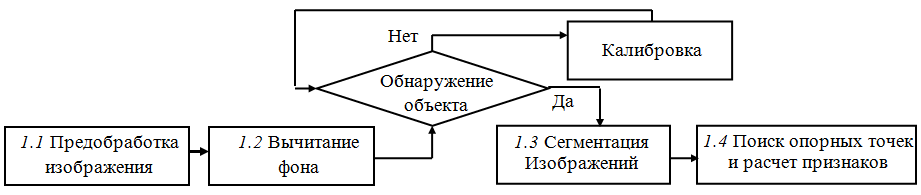
\includegraphics [width=1\linewidth] {images/h53.png}
\begin{center}
%\captionsetup{justification=justified, labelsep=period}
\caption{Блок-схема процесса извлечения антропометрических признаков.} \label{img53}
\end{center}
\end{figure}

\textit{1.1 Предварительная обработка изображения (п.2.2.1).} На этом этапе происходит преобразование входного изображения из формата RGB в полутоновое изображение. Предварительная обработка изображений: необходимо подавить шум, выполнить сглаживание изображения, провести эквализацию гистограммы, применить морфологические операторы для улучшения качества контура объекта.

\textit{1.2 Обнаружение объектов (п.2.2.2).} На этом шаге первым делом выполняется вычитание фона (C. Stauffer 1999). Результатом является область изображения, которая содержит человеческое тело (область интереса - ROI). К извлеченной области далее будет применена сегментация. Отбор пикселей, принадлежащих фону и объекту проводится с использованием бинарного изображения (маски). Считается, что пиксель принадлежит объекту и имеет белый цвет в маске, если разность интенсивности фона и текущего кадра для данного пикселя превышает некоторое пороговое значение.

\textit{1.3 Сегментация изображений на основе метода разрезов на графах (Y. Boykov 2004) (п.2.2.3).}

\begin{figure}[ht!]
\centering
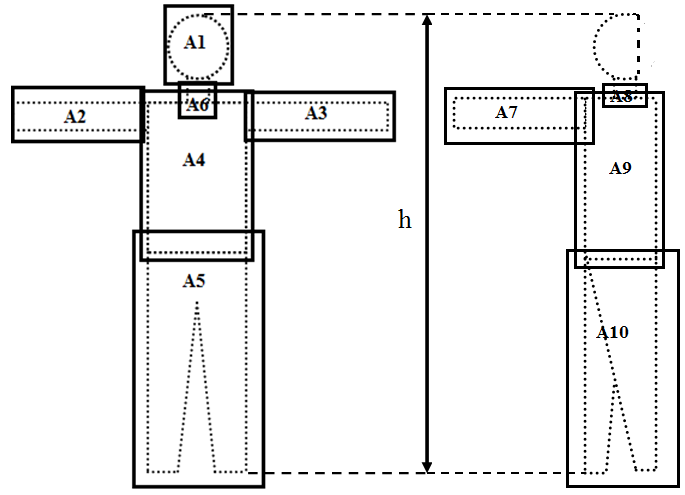
\includegraphics [width=0.45\linewidth] {images/h111.png}
\begin{center}
%\captionsetup{justification=justified, labelsep=period}
\caption{Моделирование телосложения для сегментации изображения. h (рост) - параметр калибровки.} \label{img1}
\end{center}
\end{figure}
Предположим, что множество $S=\left\{s_i|i=1, ..., n\right\}$ представляет собой область интереса, которую получили после вычитания фона.
Сегментация определяется набором случайной величины $A=\left\{A_i|i=1, ..., n\right\}$, $A_i\in L $ которого указывает маркировка $s_i$ и $L=\left\{L_j|j=1, ..., m\right\}$ является набором меток.

Каждый ROI имеет области, которые содержит части человеческого тела: голова, шея, руки, ноги и тело. Проводится калибровка с учетом параметров камеры и параметра h (см. рис. \ref{img1}). Одним из эффективных методов сегментации является метод минимального разреза - максимального потока. В этом случае алгоритм трактует всё изображение как граф $G\left(V, E\right)$. Элементы множества $V$ называются вершинами-пикселями графа, а пары из $E$ — его рёбрами. В полученном графе находится минимальный разрез, который делит граф на 2 части. Пиксели, попавшие в один подграф с истоком, считаются областями частей человеческого тела, остальные пиксели признаются областями где нет частей человеческого тела. Результаты сегментации используются далее на этапе обработки и анализа контура каждой части человеческого тела.

\textit{1.4 Построение опорных точек на основе итеративного алгоритма ближайших точек (ИАБТ) (Z. Zhang 1992) (п.2.2.4).} Пусть $A=\left\{a_i| i=1, ..., n\right\}$ представляет собой набор точек контура частей человеческого тела. $B=\left\{b_i| i=1, ..., m\right\}$ является модельным набором координат для обнаружения искомых опорных точек. Цель алгоритма ИАБТ состоит в поиске набора точек доставляющих минимум расстояния между наборами А и B:

\begin{algorithm}[ht!]
  \KwData{2 облака точек $A=\left\{a_i\right\}$, $B=\left\{b_i\right\}$; начальное преобразование $T_0$}
  \KwResult{итоговое преобразование $T$ для обнаружения опорных точек в $A$,}
  $T\leftarrow T_0$\;
  \While{\texttt{не сходится}}{
	\For{\texttt{$i\leftarrow 1$ to $n$}}
     {
		$m_i \leftarrow$ Найти ближайшие точки в $A$ к $T\ast b_i$;

		\eIf{$\left\|m_i -T\ast b_i\right\|\leq d_{max}$}{
      $w_i \leftarrow 1$;
    }{
       $w_i \leftarrow 0$;
    }
   }
	$T\leftarrow argmin_{T}\left\{\sum_i w_i\left\|T\ast b_i -m_i\right\|^2\right\}$;\\
	$n=n+1$;
		}
  \caption{Описание алгоритма ИАБТ.}
\end{algorithm}

Поиск итогового расположения опорных точек на найденных опорных контурах для каждой ROI (рис. \ref{img1}) осуществляется согласно ГОСТ$^4$. Результаты обнаружения опорных точек представлены на рис. \ref{img7}.
\begin{figure}[ht!]
\centering
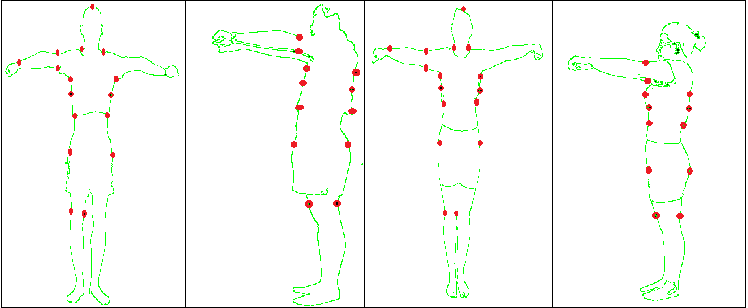
\includegraphics [width=0.9\linewidth] {images/h18.png}
\begin{center}
%\captionsetup{justification=justified, labelsep=period}
\caption{Результаты обнаружения опорных точек.} \label{img7}
\end{center}
\end{figure}
Расчеты проводятся с использованием евклидова расстояния. С такими антропометрическими признаками, как длина руки, длина плеча и т.д. (несложная геометрия) использовалось непосредственно евклидово расстояние между соответствующими опорными точками. Для извлечения антропометрических признаков со сложной структурой (талия, грудь, бедро) необходимо было использовать больше опорных точек и вычислить периметр вписанных замкнутых кривых (рис. \ref{img2}).

\begin{figure}[ht!]
\centering
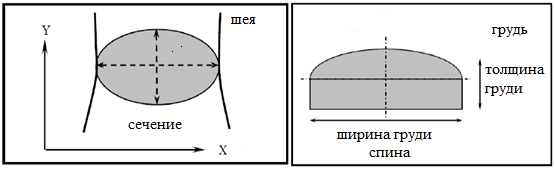
\includegraphics [width=0.8\linewidth] {images/h2.png}
\begin{center}
\caption{Примеры расчетов для обхвата шеи и груди.} \label{img2}
\end{center}
\end{figure}
\textit{1.5 Экспериментальное оценивание точности численного метода извлечения антропометрических признаков (п.2.3).} Оценка точности извлеченных признаков проведена использует анализ относительной среднеквадратической ошибки:
\begin{equation}\label{eq26}
\varepsilon_{rel}=\left\{\frac{\sum^{12}_{j=1}\left(\widetilde{z}_j - z_j\right)^2}{\sum^{12}_{j=1}z_j^2}\right\}^{1/2} = \frac{\left\|\widetilde{z} -z\right\|_2}{\left\|z\right\|_2},
\end{equation}
где $z_j$ -- результат измерений, рассчитанных вручную;
$\widetilde{z_j}$ -- результат измерений с помощью разработанного приложения. Использовалась база из 100 тестовых наборов изображений людей различного пола и телосложения. Кроме того, проведен подробный анализ ошибок измерений $\varepsilon = \left|\widetilde{z_j} - z_j\right|$ (см. рис. \ref{img16}а), при этом в первом случае использованы 24 опорных точек, а во втором - 28 точек. Экспериментально установлено, что  распределение случайной составляющей погрешности измерений (рис. \ref{img16}б) подчинено нормальному закону. В этом разделе также экспериментально установлена линейная сходимость предложенного численного метода на основе анализа апостериорной оценки погрешности при увеличении разрешения исходных изображений.
\begin{figure}[ht!]
\centering
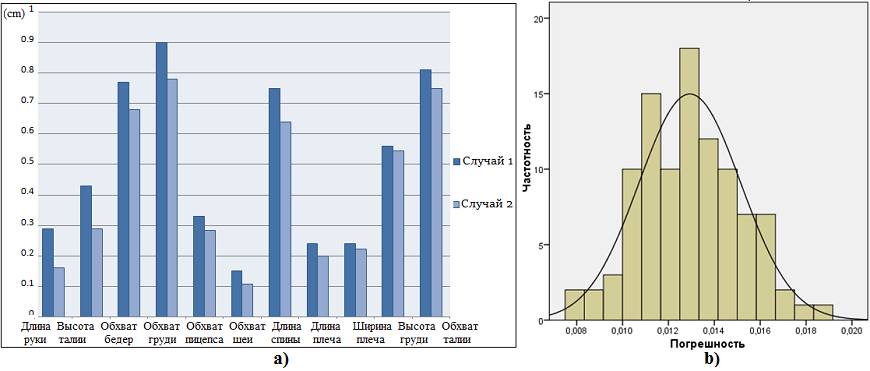
\includegraphics [width=0.96\linewidth] {images/h16.png}
\begin{center}
\caption{а) Погрешность $\varepsilon$. б) закон распределения погрешности измерений (сл. 2) по формуле (\ref{eq26}).} \label{img16}
\end{center}
\end{figure}

\textbf{2. Математическое моделирование типов телосложения.} Для построения 3D моделей экспериментальным путем было выявлено пять характеристических типов телосложения, по которым проводилась классификация. Каждый тип телосложения в свою очередь позволил строить 5 моделей. Кратко изложим адаптированную математическую модель для классификации антропометрических данных с помощью алгоритма случайного леса (Random Forest) (L. Breiman 2001). Пусть задан набор объектов $D=\left\{d_i|i=1, ..., N\right\}$, $X=\left\{x_i|i=1, ..., 12\right\}$ - набор антропометрических вектор-признаков и $Y=\left\{y_i|i=1, ..., 5\right\}$ - набор меток классов. Векторы антропометрических признаков $\left\{X_i\right\}^N_{i=1}$, в том числе каждый вектор имеет структуру $x_k=\left(x_{k1}, ..., x_{kd}\right)$. Модель обучения и тестирования использована для классификации объектов по меткам $Y$. Для оценки критерия качества построения решающих деревьев используется индекс Джини:
\begin{equation}\label{eq27}
Gini=N_L\sum^k_{i=1} p_{kL} \left(1-p_{kL}\right) + N_R\sum^k_{i=1} p_{kR} \left(1-p_{kR}\right),
\end{equation}
где $p_{kL}$ -- доля класса $K$ в левом узле ($N_L$), $p_{kR}$ -- доля класса $K$ в правом узле ($N_R$).
Предлагается алгоритм оценки и поиска набора признаков из исходного набора признаков. Алгоритм случайного леса состоит из двух основных этапа: обучение и тестирование. Процесс обучения осуществляется следующим образом:

\begin{itemize}
	\item взять из $D$ $n$ случайных объектов с повторениями (bootstrap sample) - $D_i$;
	\item построить для $D_i$ дерево, используя алгоритм <<дерево классификации и регрессии>> (CART) для построения решающего дерева. Причем для каждой вершины признак выбирается из $m$ случайно выбранных ($m$ - параметр, $1\leq m\leq p$);
	\item дерево строится до конца, без отсечения ветвей;
	\item повторить предыдущие шаги $B$ раз.
\end{itemize}
В итоге строится $B$ деревьев. Для проверки новых наборов антропометрических данных используются модели обучения.

\textbf{3. Задача построения антропометрических моделей.} В этом разделе представлен подход к реконструкции 3D-
\begin{figure}[ht!]
\centering
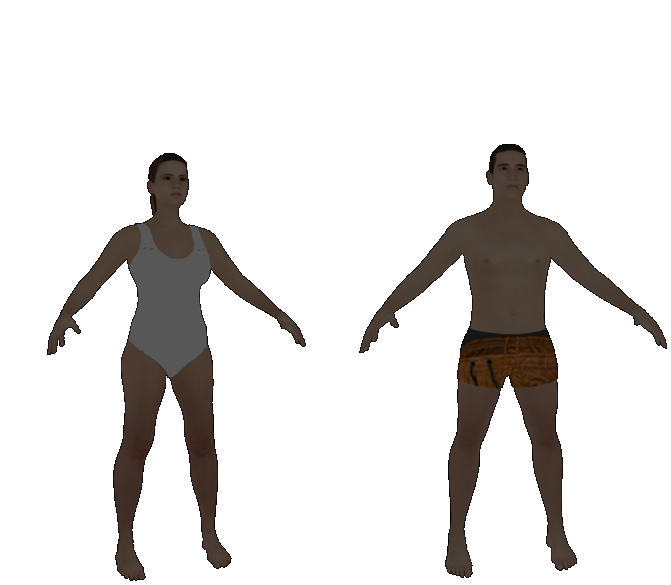
\includegraphics [width=0.6\linewidth] {images/h22.png}
\begin{center}
%\captionsetup{justification=justified, labelsep=period}
\caption{Примеры построенных моделей.} \label{img17}
\end{center}
\end{figure}
модели человека на основе антропометрических признаков, которые были предварительно извлечены и классифицированы. Использован набор данных антропометрических признаков для построения 3D-моделей телосложения.

Процесс построения антропометрических моделей включает следующие шаги:

	\textbf{ Шаг 1}: описание текстурных характеристик человеческого тела, а также текстуры одежды;

   \textbf{Шаг 2}: разработка моделей частей человеческого тела (голова, туловище, руки, ноги) с использованием ранее полученных антропометрических признаков;

\textbf{Шаг 3}: построение текстурированной модели человеческого тела;

\textbf{Шаг 4}: экспорт модели человеческого тела в два файла: первый файл (*.mtl) описывает текстуры модели, второй файл (*.obj) содержает информацию каждой модели. На рис. \ref{img17} представлены примеры построения антропометрических моделей.

В \textbf {третьей главе} описывается проектирование системы компьютерного зрения в антропометрии для практических применений: моделирование одежды и фитнес-приложение. Система проектируется с помощью аналитических методов объектно-ориентированного UML (рис. \ref{img35}). Программа описывается диаграммами: диаграмма прецедентов, диаграмма классов, диаграмма последовательности. Классы подробно анализируются с указанием задач каждого компонента в программе. Доказывается целесообразность проектирования приложений компьютерного зрения в антропометрии.
\begin{figure}[ht!]
\centering
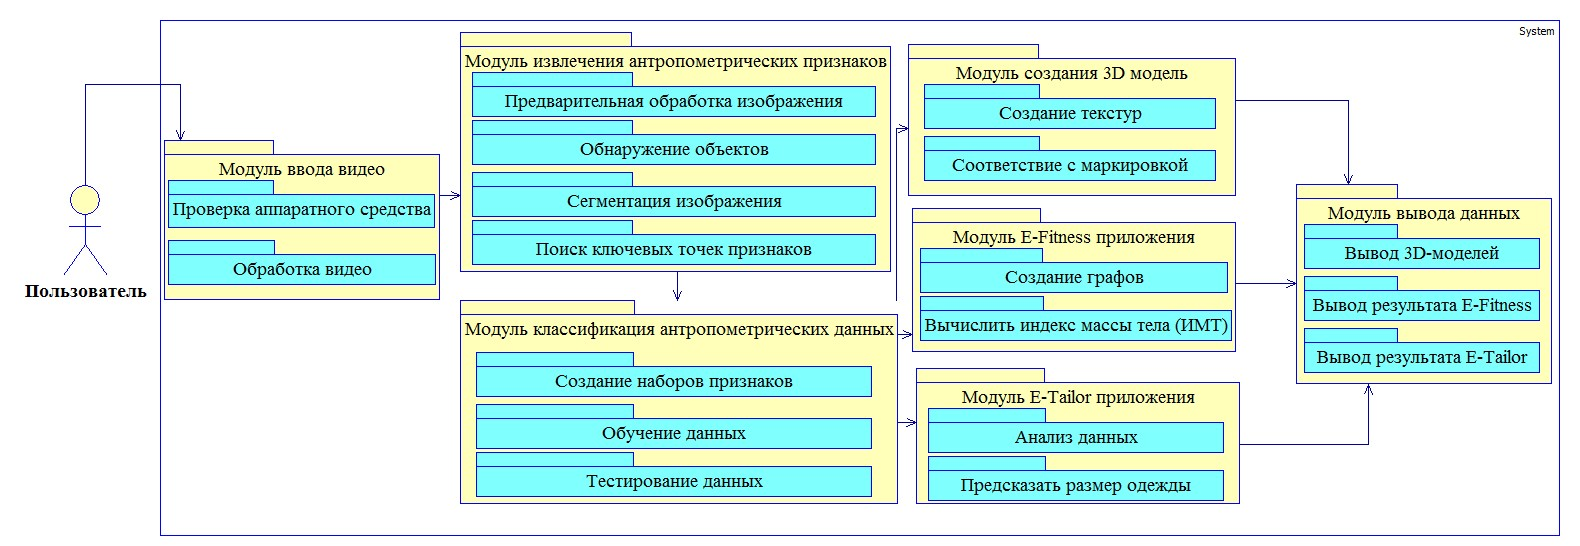
\includegraphics [width=0.95\linewidth]{images/h35.png}
\begin{center}
%\captionsetup{justification=justified, labelsep=period}
\caption{Структура ПО.} \label{img35}
\end{center}
\end{figure}

Проведен анализ практических результатов экспериментов извлечения антропометрических признаков. Выполнено сравнение результатов предложенных алгоритмов с другими алгоритмами по точности. Установлено преимущество синтеза алгоритма на основе метода разреза на графах и итеративного алгоритма ближайших точек. И наконец, выполнено сравнение результатов классификации между алгоритмом случайного леса и алгоритмом Boosting, работающими с видео.

В \textbf{четвертой главе} дано описание среды разработки приложения Android, библиотек поддержки алгоритмов компьютерного зрения OpenCV\footnote{OpenCV - Open source computer vision [Electronic resource] // [http://opencv.org/] -- [S. l. : s. n.]. -- Дата доступа: 2017.}, поддержки построения 3D-моделей человеческого тела MakeHuman\footnote{MakeHuman library [Electronic resource] // [http://www.makehuman.org]. -- USA: [s. n.]. -- Дата доступа: 2017.} и библиотеки поддержки 3D для Android – Min3D\footnote{Softpedia. Min3D library [Electronic resource] // [https://code.google.com/p/min3d]. -- USA: [s. n.]. -- Дата доступа: 2017.}. Изложены инструкции для пользователей разработанных приложений. Приведена архитектура мобильного приложения для моделирования одежды (E-Tailor). Главные функции приложения включают: автоматизацию извлечения антропометрических признаков и классификацию размеров одежды. Изложены этапы разработки приложения для фитнеса (E-Fitness). Главные функции разработанного приложения включают: автоматизацию извлечения антропометрических признаков, построение 3D-моделей человеческого тела, анализ и сравнение признаков телосложений, а также расчет индекса массы тела (ИМТ). Приложения разработаны на языке Java под ОС Android для смартфонов. Программные модули имеют простой, удобный и интуитивно понятный интерфейс.

\textbf{
\begin{center}
ОСНОВНЫЕ РЕЗУЛЬТАТЫ ДИССЕРТАЦИОННОЙ РАБОТЫ
\end{center}
}

\begin{enumerate}
	\item[1)] Разработаны алгоритмы компьютерного зрения для извлечения антропометрических признаков, основанные на комбинации алгоритма сегментации изображений на основе метода разрезов на графах и итеративного алгоритма ближайших точек;
	\item[2)] Предложена модель и разработан и апробированы алгоритм классификации антропометрических данных методом случайного леса (Random Forest) для приложения, которое классифицирует объекты на основе антропометрических признаков;
	\item[3)] Разработаны алгоритмы и методы компьютерного зрения к задаче антропометрии на изображениях и видео с наличием шума и в режиме реального времени;
	\item[4)] Построены антропометрические модели человеческого тела на основе результата извлечения антропометрических признаков;
	\item[5)] Разработанные алгоритмы и методы реализованы в виде двух приложений для смартфонов на ОС Android: приложение «E-Tailor» для моделирования одежды и приложение «E-Fitness» для фитнес-тестирования.
\end{enumerate}
\textbf{
\begin{center}
СПИСОК ОСНОВНЫХ РАБОТА ПО ТЕМЕ ДИССЕРТАЦИИ
\end{center}
}

\textbf{Издания, входящие в Перечень ВАК РФ:}

\begin{enumerate}
	\item Нгуен~Т.Л. Об автоматизации извлечения и классификации антропометрических признаков / Нгуен Т.Л., Нгуен Т.Х. // Вестник ИРНИТУ: №~4. 2015. -С. 17-23.
	\item  Nguyen~T.L. Studies of Anthropometrical Features using Machine Learning Approach / Nguyen T.L., Nguyen T.H., A. Zhukov // CEUR Workshop Proceedings. 2015, -V. 1452, -P. 96-105.
	\item Нгуен~Т.Л. О распознавании и классификации дефектов дорожного покрытия на основе изображений / Нгуен Т.Л., Нгуен Т.Х. // Вестник ИРНИТУ: №~10. 2016. -С. 111-118.
	\item Nguyen~T.L. Automatic Anthropometric System Development Using Machine Learning / Nguyen T. L., Nguyen T.H. // BRAIN. Broad Research in Artificial Intelligence and Neuroscience. 2016, -V. 7, -P. 5-15.\\
	\textbf{Издания, включенные в РИНЦ:}
	\item Nguyen T.H. A Robust Approach for Defects Road Pavement Detection and Classification/ Nguyen T. L., Nguyen T.H., D. N. Sidorov // Journal of Computational and Engineering Mathematics: 2016,-V. 3.-No. 3. -P. 40-52.\\
	\textbf{Свидетельства о государственной регистрации программы для ЭВМ:}
	\item  Сидоров Д.Н. Программа бесконтактной антропометрии для смартфонов на операционной системе Андроид // Сидоров Д.Н., Нгуен Т.Л., Нгуен Т.Х. // Свидетельство о гос. регистрации программы для ЭВМ. № 2016611475, от 03 февраля 2016 г. М.: Федеральная служба по интеллектуальной собственности. 2016.
	\item  Сидоров Д.Н. Программа автоматического обнаружения и классификации дефектов дорожного покрытия // Сидоров Д.Н.,  Нгуен Т.Х., Нгуен Т.Л. // Свидетельство о гос. регистрации программы для ЭВМ. № 2016619386, от 18 августа  2016 г. М.: Федеральная служба по интеллектуальной собственности. 2016.\\
\textbf{Прочие издания:}
\item  Нгуен Т.Л. Автоматизация антропометрических измерений и извлечение признаков из 2D-изображений / Нгуен Т.Л., Нгуен Т.Х. // Байкальская международная школа-семинар <<методы оптимизации и их приложения>>. О. Ольхон, Иркутск 2014г. -С. 153.
\item Нгуен Т.Л. Построение программы для обнаружения контуров человека в изображении с помощью методов математической морфологии / Нгуен Т.Л., Нгуен Т.Х. // Материалы всероссийской молодежной научно-практической конференции <<Винеровские чтения 2014>>. Иркутск: Изд-во Иркутск, 2014. -С 10.
\item Нгуен Т.Л. Классификация и кластерный анализ антропометрических признаков / Нгуен Т.Л.// Материалы всероссийской молодежной научно-практической конференции <<Винеровские чтения 2015>>. Иркутск: Изд-во Иркутск, 2015. -С.8.
\item Нгуен Т.Л. Методы математической морфологии в цифровой обработке изображений / Нгуен Т.Л., Нгуен Т.Х. // Труды XIX Байкальской Всероссийской конференции <<информационные и математические технологии в науке и управлении>>. Иркутск: ИСЭМ СО РАН, 2014. -С. 75-81.
\item Нгуен Т.Л. Анализ антропометрических признаков с использованием методов машинного обучения / Нгуен Т.Л., Нгуен Т.Х. // Междисцплинарные исследования в области математического моделирования и информатики . Ульяновск: Изд-во SIMJET, января 2015г.-С.204-210.
\item Nguyen T.L. On Road Defects Detection and Classification / Nguyen T.L., Nguyen T.H., A. Zhukov // Supplementary Proceedings of the 5th International Conference on Analysis of Images, Social Networks and Texts (AIST 2016). CEUR Workshop Proceedings, 2016,-V. 1710, -P. 266- 278.
\end{enumerate}
         % Содержание автореферата

\end{document}